\documentclass[10pt,a4paper]{article}
\usepackage[utf8]{inputenc}
\usepackage[english]{babel}
\usepackage[left=2cm,right=2cm,top=2cm,bottom=2cm]{geometry}
\usepackage[hyphens]{url}
\usepackage{hyperref}
\usepackage{listings}
\usepackage{amsmath}
\usepackage{amsfonts}
\usepackage{amssymb}
\usepackage{color}
\usepackage{subfigure}
\usepackage{graphicx}
\graphicspath{{Figures/}}
\author{Pierre Lecomte \\ \textit{ \href{mailto:pierre.lecomte@gadz.org}{pierre.lecomte@gadz.org}}}
\title{ambitools Documentation}

%%% MY COLORS
\definecolor{yoheader}{rgb}{0.71,0.01,0.0}

%%%% margin par
\definecolor{margincolor}{rgb}{0.52,0.02,0.02} % grey red.
\definecolor{yobg}{rgb}{0.9,0.9,1}
\definecolor{yotxt}{rgb}{0.01,0.01,0.52}
\definecolor{mylstcmt}{rgb}{0.01,0.52,0.01} % a dark green.
%\definecolor{mylstdoc}{rgb}{0.60,0.60,0.60} % a medium grey.
\definecolor{mylstdoc}{rgb}{0.80,0.30,0.80} % a medium pink.
%\definecolor{mylsteqn}{rgb}{0.80,0.80,0.30} % a medium pink.
\definecolor{mylstkey}{rgb}{0.52,0.01,0.01} % a dark red.
%%\newcommand{\farg}[1]{\textrm{\textit{#1}}}

\begin{document}

\lstset{
  tabsize=4,
  showspaces=false,
  showstringspaces=false,
  %language=C++, 
  basicstyle=\ttfamily\color{yotxt},
  numbers=none,
  stepnumber=2,
  commentstyle=\slshape\color{mylstcmt},
  breaklines=true, 
  emph={Gain,Radius,Azimuth,Elevation,Spherical, Wave, Speakers,Mute,NFC,Outputs,Inputs,left,right,front,back,up,down,Order,Output},
  emphstyle=\color{mylstkey},
%  morecomment=[s][\color{mylsteqn}]{<equation>}{</equation>},
  morecomment=[s][\color{mylstdoc}]{<mdoc>}{</mdoc>},
  %% frame=single,
  backgroundcolor=\color{yobg},
  captionpos=b
}

\makeatletter
\newcommand\footnoteref[1]{\protected@xdef\@thefnmark{\ref{#1}}\@footnotemark}
\makeatother

\maketitle
\tableofcontents
\section{Introduction}

\subsection{Goals of ambitools}
ambitools is a collection of tools for sound-field synthesis using Near-Field Compensated Higher Orders Ambisonics (NFC-HOA). For the rest of this document, the denomination Ambisonics will be used for simplicity.
ambitools is developped in the context of my PhD on 3D sound field synthesis. The audio processing is coded in \textsc{Faust}\footnoteref{faustlive} (Functional AUdio Stream) which allows to produce efficent C++ code and exports in various DSP tools format : VST, standalone applications, LV2, etc. Thus, ambitools is multi-platform (although conceived under Linux/Jack).

The goal of ambitools is mainly to produces several modules to encode, decode and transform 3D synthesized sound field or 3D recordings in a context of physical sound field synthesis. 

The project is open-source under GPL licence. ambitools is thought to be very flexible to adapt to your configuration. The \textsc{Faust}-code for each tools has an header with the required order. So, for example, if you need an encoder up to order $M=4$, for $N=5$ sources, you just has to change this two parameters in \lstinline'hoa_encoder_N_sources.dsp' and produce de required plug-in using \textsc{FaustLive}\footnote{\label{faustlive}\url{http://faust.grame.fr}} for example.

Don't hesitate to contact me for any suggestions, requirements, critics or even just to tell me you're using ambitools !

\begin{flushright}
Pierre Lecomte
\end{flushright}

\subsection{Ambisonics overview}
This section presents the basis of Ambisonics for 3D sound field synthesis. It is written with relatively few maths to focus on the concepts instead of the mathematical rigor, which would be out of scope of this document. If you want more insights to Ambisonics refer for example to \cite{daniel2000representation,poletti2005three,ahrens2012analytic}.

\subsubsection{Principles}
Ambisonics are some mathematical approaches to represent a sound field in two or three dimensions over a basis of spherical harmonics. Without giving more mathematical details, Ambisonic main possibilities are displayed on Fig.~\ref{fig:ambisonics}.
\begin{figure}[!ht]
	\centering
	\def\svgwidth{\columnwidth}
	\input{Figures/Fig_Apercu_Ambisonics.pdf_tex}
	\caption{Ambisonic principles: A sound field can be captured in three dimensions using spherical microphone or it can be synthesized with monophonic signals and explicit positions in space. These two approaches result in an encoded sound field in Ambisonic domain up to order $M$. In this domain, transformations can be done such as: sound field mirroring, rotation, warping, directional filtering, etc. Finally, the decoding step computes the driving signals of the playback loudspeakers to recreate the encoded sound field in a sweet spot region of space. The decoding can be done over various configurations of speakers and even over headphones !}
	\label{fig:ambisonics}
\end{figure}

Thus, in accordance to this Fig.~\ref{fig:ambisonics}, ambitools provides tools to:
\begin{itemize}
\item Encode a sound field captured by a spherical microphone.
\item Encode a sound field from monophonic signals and explicit position in space.
\item Transform and manipulate the encoded sound field in Ambisonic domain.
\item Decode the sound field over spherical grids of speaker or over headphones with binaural convolution.
\end{itemize}

\subsubsection{Spherical coordinate system}
\label{sec:spherical_coordinates}
Ambisonics are usually described in spherical coordinate systems. In ambitools, the following spherical coordinate system is used:
The following spherical coordinate system is used and is shown in Fig.~\ref{fig:coord_sph}:
\begin{equation}
x = r \cos(\theta) \cos(\delta), \; y = r \sin(\theta) \cos(\delta), \;
z = r \sin(\delta)\textcolor{red}{.}
\end{equation}
\begin{figure}[ht]
\centering
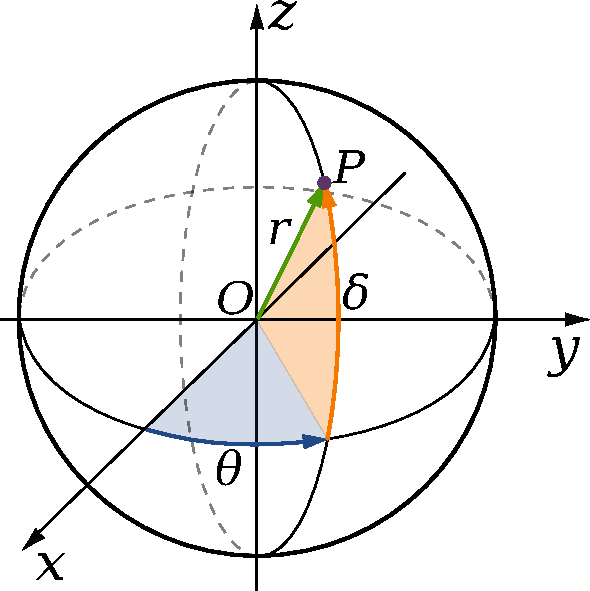
\includegraphics[height=0.3\columnwidth]{Fig_Coord_Sph.pdf}
\caption{Spherical coordinate system in use. A point $P (x,y,z)$ is described by radius $r$, azimuth $\theta$ and elevation $\delta$.}
\label{fig:coord_sph}
\end{figure}
The azimuth angle $\theta \in [0~~360^\circ]$. The elevation angle $\delta \in [-90^\circ~~90^\circ]$. The convention for rotation is counterclockwise direction (i.e. trigonometric direction).

\subsubsection{Spherical harmonics}
As mentionned before, Ambisonics describes a sound field over a spherical harmonics basis. Those functions are directional functions of the variable $\theta,\delta$. They are denoted $Y_{mn}(\theta,\delta)$ where subscript $m$ represent the order of the spherical harmonic and $n$ its degree. There is several definition for these functions. In ambitools, the N3D real spherical harmonic definition is used \cite{daniel2000representation}:
\begin{equation}
Y_{mn}(\theta,\delta) = \sqrt{(2m+1)\epsilon_n \frac{(m-|n|)!}{(m+|n|)!}} P_{m|n|}(\sin(\delta))
 \times \left\lbrace \begin{aligned} \cos(|n| \theta) & & \text{if} & & n \geq 0 \\ \sin(|n| \theta)  & & \text{if} & & n < 0  \end{aligned} \right.,
\label{eq:ymn}
\end{equation}
where $P_{m|n|}$ are the associated Legendre polynomials of order $m$ and degree $|n|$, $(m,n) \in (\mathbb{N},\mathbb{Z})$ with $|n| \leq m$, and $\epsilon_n = 1$ if $n = 0$, $\epsilon_n = 2$ if $|n| > 0$. In Eq.~\eqref{eq:ymn}, $m$ denotes the spherical harmonic order and $n$ its degree.

For each order $m$, there are $(2 m +1)$ spherical harmonics. Thus a basis truncated at order $M$ contains $(M+1)^2$ functions. For example, on Fig.~\ref{fig:spherical_harmonics} are displayed the spherical harmonics up to order $M=5$ as balloon plots.

Thus, a sound field can be described as a linear combination of spherical harmonics. The weights of this linear combination are called the Ambisonics components or $B$-Format components. As an example, a sound field described up to order $M=1$ is described with $(M+1)^2=4$ Ambisonics components. At order $M=5$ there will be $36$ components, etc.

Without giving more details, the concept to retain is that the more components are available to describe the sound field (i.e. the higher the order), the larger the sweet-spot will be on Fig.~\ref{fig:ambisonics}.

At the moment, ambitools offers the possibility of 3D Ambisonics up to order $M=5$. Thus for all the tools you need to compile, \textcolor{red}{\textsc{$M$ should be chosen such as $M \leq 5$.}}

\begin{figure}[ht]
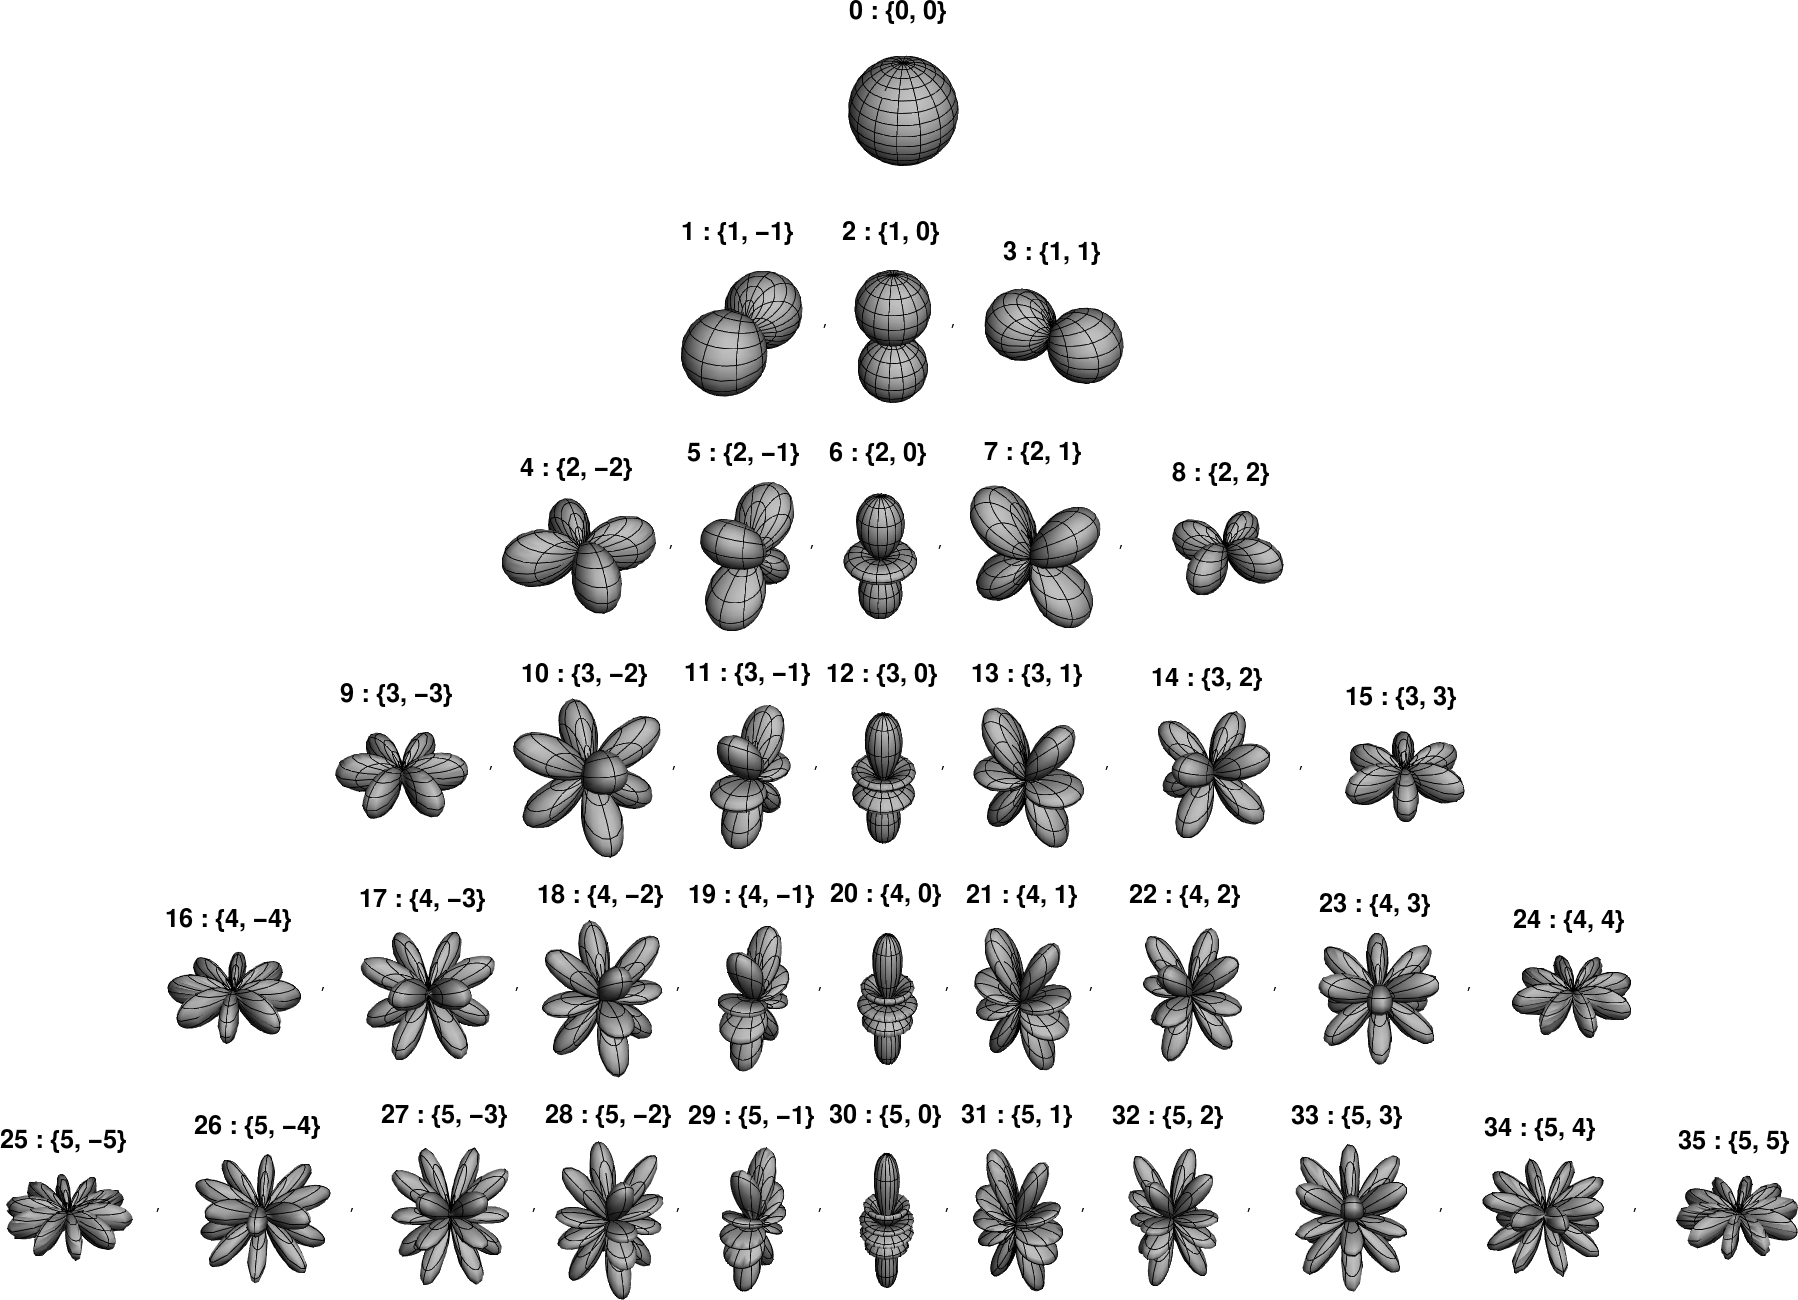
\includegraphics[width=\columnwidth]{Fig_YACN.png}
\caption{Balloon-plot of the spherical harmonics up to order $M=5$.}
\label{fig:spherical_harmonics}
\end{figure}

\pagebreak
\section{Installing ambitools}

\subsection{Retrieve ambitools repository}
To install ambitools, simply go on the github repository\footnote{\url{https://github.com/sekisushai/ambitools}} and clone it. To do so, open a terminal in the directory you'd like to clone the repository and type the following command:

\begin{lstlisting}
$ git clone https://github.com/sekisushai/ambitools
\end{lstlisting}

To keep the repository up to date, type the following command at the root of the directory \lstinline`ambitools/`:

\begin{lstlisting}
$ git pull
\end{lstlisting}

You can also download a \lstinline'.zip' file from github\footnote{\url{https://github.com/sekisushai/ambitools/archive/master.zip}}

The resulting \lstinline'ambitools/' folder should have the following structure:

\begin{itemize}
    \item \lstinline'Documentation/' Everything concerning the documentation (pdfs, including some scientific papers).
    \item \lstinline'Faust/' Everything written in \textsc{Faust} language (all the ambitools plug-ins + some utilities).
    	\subitem \lstinline'bin/' Compiled plug-ins in various formats.
    	\subitem \lstinline'src/' Source code of the plug-ins.
    	\subitem \lstinline'src/lib/' Shared libraries (spherical harmonics, gui, etc.).
    \item \lstinline'FIR/' Finite Impulse Response (FIR) filters banks for binaural rendering and spherical microphone equalization filters, to use with Jconvoler\footnote{\url{http://kokkinizita.linuxaudio.org/linuxaudio/}}, fast convolution software.
    	\subitem \lstinline'spherical_microphones/' Equalization filters for rigid spherical microphone, such as mh acoustics EigenMike\textsuperscript{\textregistered}\footnote{\url{http://www.mhacoustics.com}}
  		\subitem \lstinline'hrir/' Head Related Impulses Responses (HRIR) of several people to use with binaural rendering over headphones.
    \item \lstinline'Processing/' Everything written in \textsc{Processing} language, namely the spherical VU-Meter ((see Sec.~\ref{sec:processing}).
    	 \subitem \lstinline'bin/' Compiled spherical VU-Meter in Java for various architectures.
    	 \subitem \lstinline'src/' \textsc{Processing} source code.
    \item \lstinline'PureData/' Everything written in Pure Data (a few sounds generator patches, head-tracking patch and PlayStation-like remote patch to drive \textsc{Faust} plug-ins with Open Sound Control protocol, OSC).
\end{itemize}

\subsection{Dependencies}
Depending on what you're looking for with the code, the following dependencies should be provided:
\begin{table}[!ht]
\centering
\begin{tabular}{|c|c|}
\hline 
Dependency & Usage \\ 
\hline 
\textsc{Osc} support & Drive the tools standalone tools with OSC. \\
\hline
\textsc{Java} & Run the Spherical VU-Meter (see Sec.~\ref{sec:processing}). \\
\hline
\textsc{Jconvolver} & Real-time convolution for binaural rendering or spherical microphone signals filtering.\\
\hline
\textsc{Processing} & Edit and compile the Processing code. \\
\hline
\textsc{Faust} or \textsc{FaustLive}  & Edit and compile the \textsc{Faust} code.\\
\hline
\end{tabular}
\caption{Dependencies of ambitools}
\end{table}

\subsection{Compile the \textsc{Faust} plug-ins}
The \textsc{Faust} plug-ins source codes are in the sub-folder \lstinline'Faust/src/'. 

\subsection{Local \textsc{Faust} installation}
If you have \textsc{Faust} installed on your machine with the required dependencies, you can run the scripts collection \lstinline'faust2*' to produce the plug-in of your choice in the desired format. 

For example, to compile \lstinline'hoa_encoder_N_sources.dsp' into a standalone Linux jack-qt application with \textsc{OSC} support, type the following command in a terminal in the folder \lstinline'\Faust/src'

\begin{lstlisting}
$ faust2jaqt hoa_encoder_N_sources.dsp -osc
\end{lstlisting}

\subsection{\textsc{FaustLive}}
To compile the plug-ins to your requirements, load the chosen plug-in in \textsc{FaustLive}\footnoteref{faustlive} and choose \lstinline'Window/Export As...' (see Fig.~\ref{fig:faustlive}).
\begin{figure}[!ht]
\centering
\includegraphics[width=0.3\columnwidth]{faustlive_export_manager.png}
\caption{\textsc{FaustLive} Export Manager}
\label{fig:faustlive}
\end{figure}

\subsection{Compile the \textsc{Processing} VU-Meter}
The \textsc{Processing} source code is in the folder \lstinline'Processing/scr'. You should open the file \lstinline'Spherical_VU_Meter.pde' in the \textsc{Processing} editor and select "File/Export..." to produce a binary application.

\section{The different tools}
This section gives a quick presentation of each tool contained in ambitools. 
\subsection{\textsc{Faust}}
The core of the sound processing is written in \textsc{Faust} language. Note that the majority of the figures presented in the following section will be screen-shots of the tools compiled as standalone \textsc{Jack} applications for Linux, using \lstinline'faust2jaqt' script. However, thanks to the versatility of \textsc{Faust} language, note that each of these tools can be compiled for various architecture, using \textsc{FaustLive}\footnoteref{faustlive} for example. 

\pagebreak
\subsubsection{hoa\_N\_sources\_encoder}
\label{sec:hoa_encoder}
\begin{itemize}
\item Inputs: $N$
\item Outputs: $(M+1)^2$
\end{itemize}

This first tool allows to encode $N$ signal inputs to an 3D Ambisonics scene described with Ambisonics components signals up to order $M$ (the $B$-Format). You can choose $N$ and $M$ at the compilation time in file \lstinline'hoa_encoder_N_sources.dsp'. The resulting graphical user interface when using \lstinline'faust2jaqt' script is shown in Fig.~\ref{fig:hoa_encoder} for $N=3, M=5$.
Each input signal can be encoded in $B$-Format as a plane wave or a spherical wave. 

For the plane wave case, the check-box \lstinline'Spherical Wave' should be unchecked. Consequently, the knob \lstinline'Radius' and input entry \lstinline'Speakers Radius' are without effect in this case (a plane wave has no distance information).

For the spherical wave case, the knob \lstinline'Radius' allows to choose the source radius to origin. Note that to represent a spherical wave in Ambisonic domain, near-field filters are activated \cite{daniel2003spatial,lecomte2015real}. Those filters, unstable by nature, are stabilized using the near-field compensation filters from decoding step. Thus in this case, the radius of the spherical loudspeakers grid should be known prior to decoding and given in \lstinline'Speakers Radius' input entry.

Finally, the outputs of this tool are $B$-Format signals up to order $M$. Each order can be muted or each individual Ambisonic components individually.

\begin{figure}[!ht]
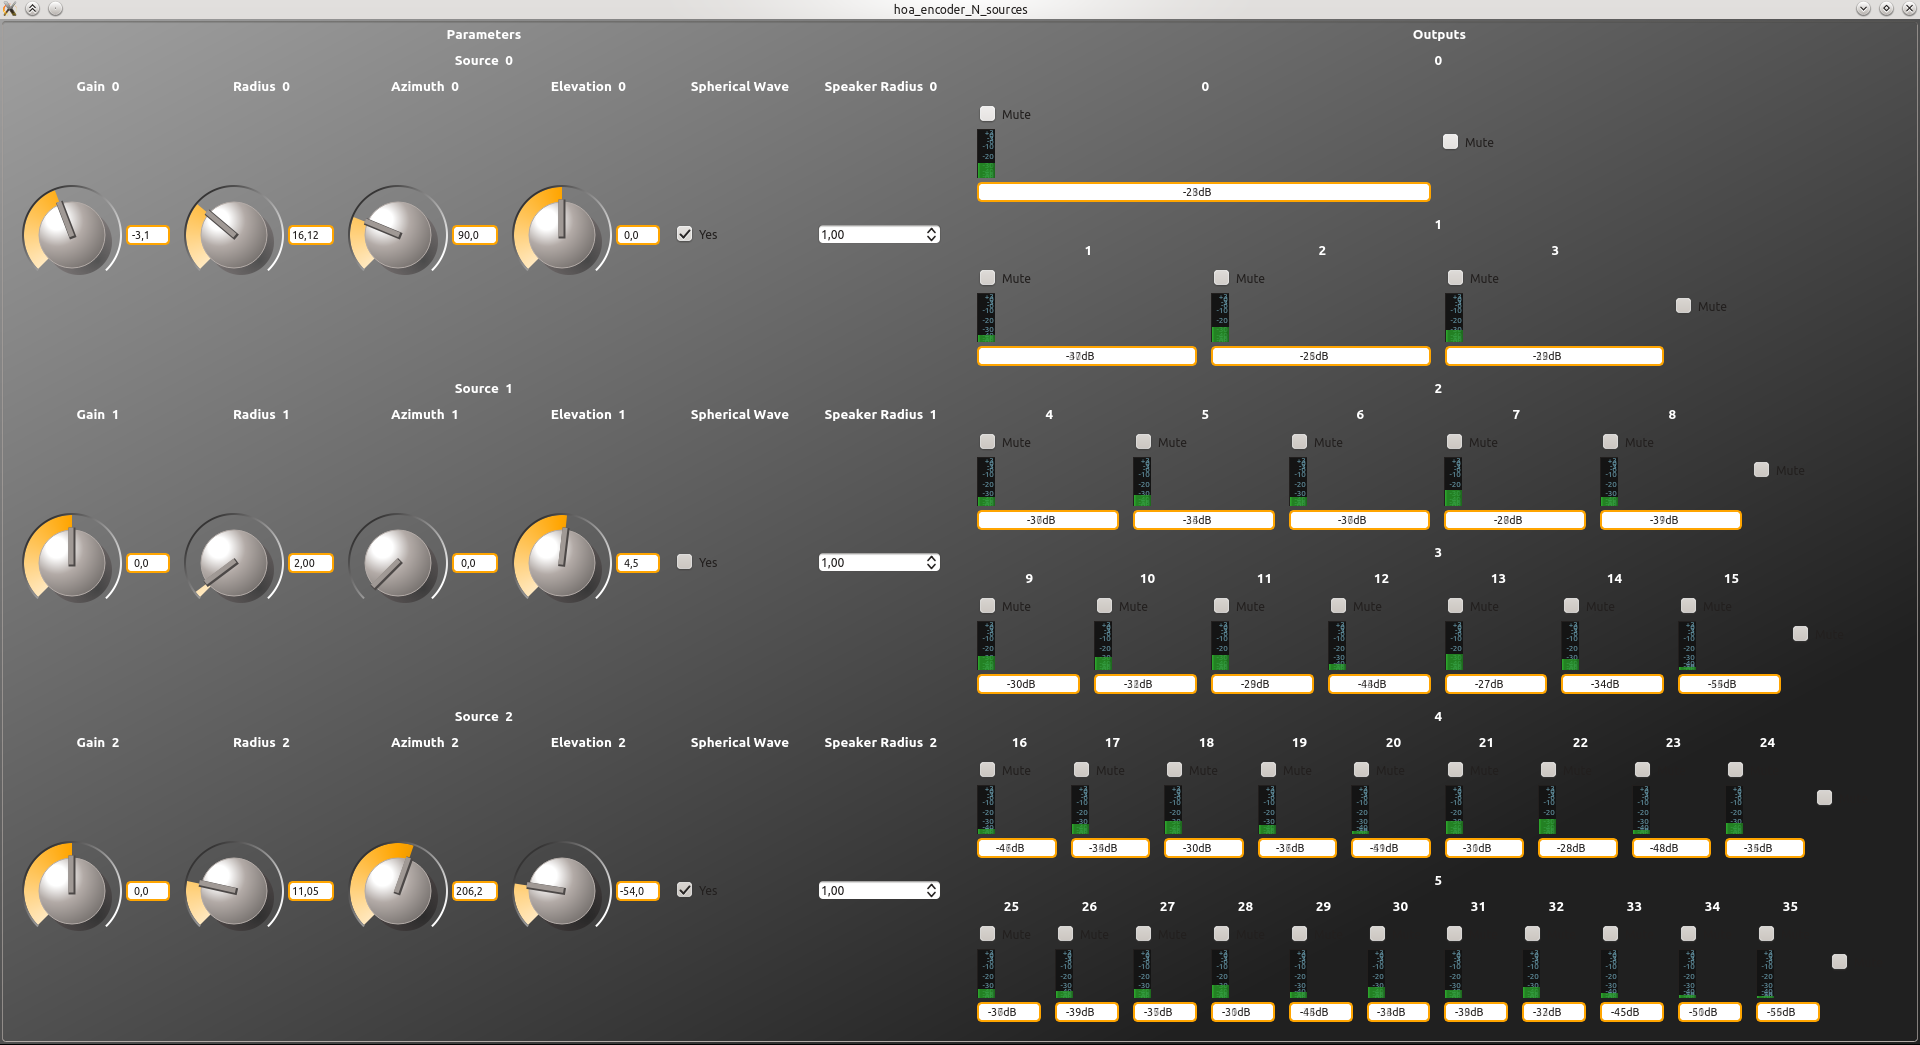
\includegraphics[width=\columnwidth]{hoa_encoder.png}
\caption{\lstinline'hoa_encoder_N_sources' plug-in compiled using \lstinline'faust2jaqt' script with $N=2$ and $M=5$. The \lstinline'Gain' knob allows to adjust the input level of the input. \lstinline'Radius' knob allows to choose the source distance to origin in case of spherical wave encoding. \lstinline'Azimuth' and \lstinline'Elevation' knobs allow to choose the source direction. The \lstinline'Spherical Wave' check-box enables the encoding of spherical wave, using near-field filters. \lstinline'Speakers Radius' sets the radius for the spherical arrays of loudspeakers at decoding stage in case of spherical wave encoding. Finally, the VU-Meters shows the level of 3D $B$-Format signals in dBFS up to order $M$. Each meter as a \lstinline'Mute' check-box and each order as well.}
\label{fig:hoa_encoder}
\end{figure}
\pagebreak

\subsubsection{hoa\_mic\_encoder*}
\begin{itemize}
\item Inputs: $06$, $26$, $32$, or $50$ depending on the configuration.
\item Outputs: $(M+1)^2$
\end{itemize}
It is possible to encode a natural sound field captured by a rigid spherical microphone, according to Fig.~\ref{fig:ambisonics}. To do so, the signals from each capsule on the spherical microphone are mixed to operate the Discrete Spherical Fourier Transform (DSFT) \cite{moreau20063d}. Then, the resulting $(M+1)^2$ components are filtered to obtain the Ambisonics components. In ambitools, the DSFT projection is done for several spherical rigid spherical microphone configurations using \lstinline'hoa_mic_encoder*' tools. The filtering of the resulting components is done using Jconvolver, a real-time fast convolution software. See Sec.~\ref{sec:jconvolver} for further details. Note that the filtering of the outputs signals of \lstinline'hoa_mic_encoder*' tools is mandatory in order to obtain the Ambisonics components.
The different microphone configuration available in ambitools are $06$, $26$ or $50$ capsules spherical microphone arranged on a Lebedev grid \cite{lecomte2015on} and a $32$ capsules spherical microphone arranged on a pentakis-dodecahedron grid, i.e. the mh acoustics Eigenmike\textsuperscript{\textregistered} microphone \cite{elko2009audio}. Those configuration can operate the Spherical Fourier Transform up to order $M=1$, $M=3$, $M=5$ and $M=4$ respectively \cite{lecomte2015on,moreau20063d}. The corresponding tools are named \lstinline'hoa_mic_encoder_lebedev06', \lstinline'hoa_mic_encoder_lebedev26', \lstinline'hoa_mic_encoder_lebedev50' and \lstinline'hoa_mic_encoder_eigenmike32' respectively. The graphical user interface when using \lstinline'faust2jaqt' script is shown in Fig.~\ref{fig:hoa_mic_encoder_lebedev26} for the \lstinline'hoa_mic_encoder_lebedev26' tool compiled with $M=3$.
\begin{figure}[!ht]
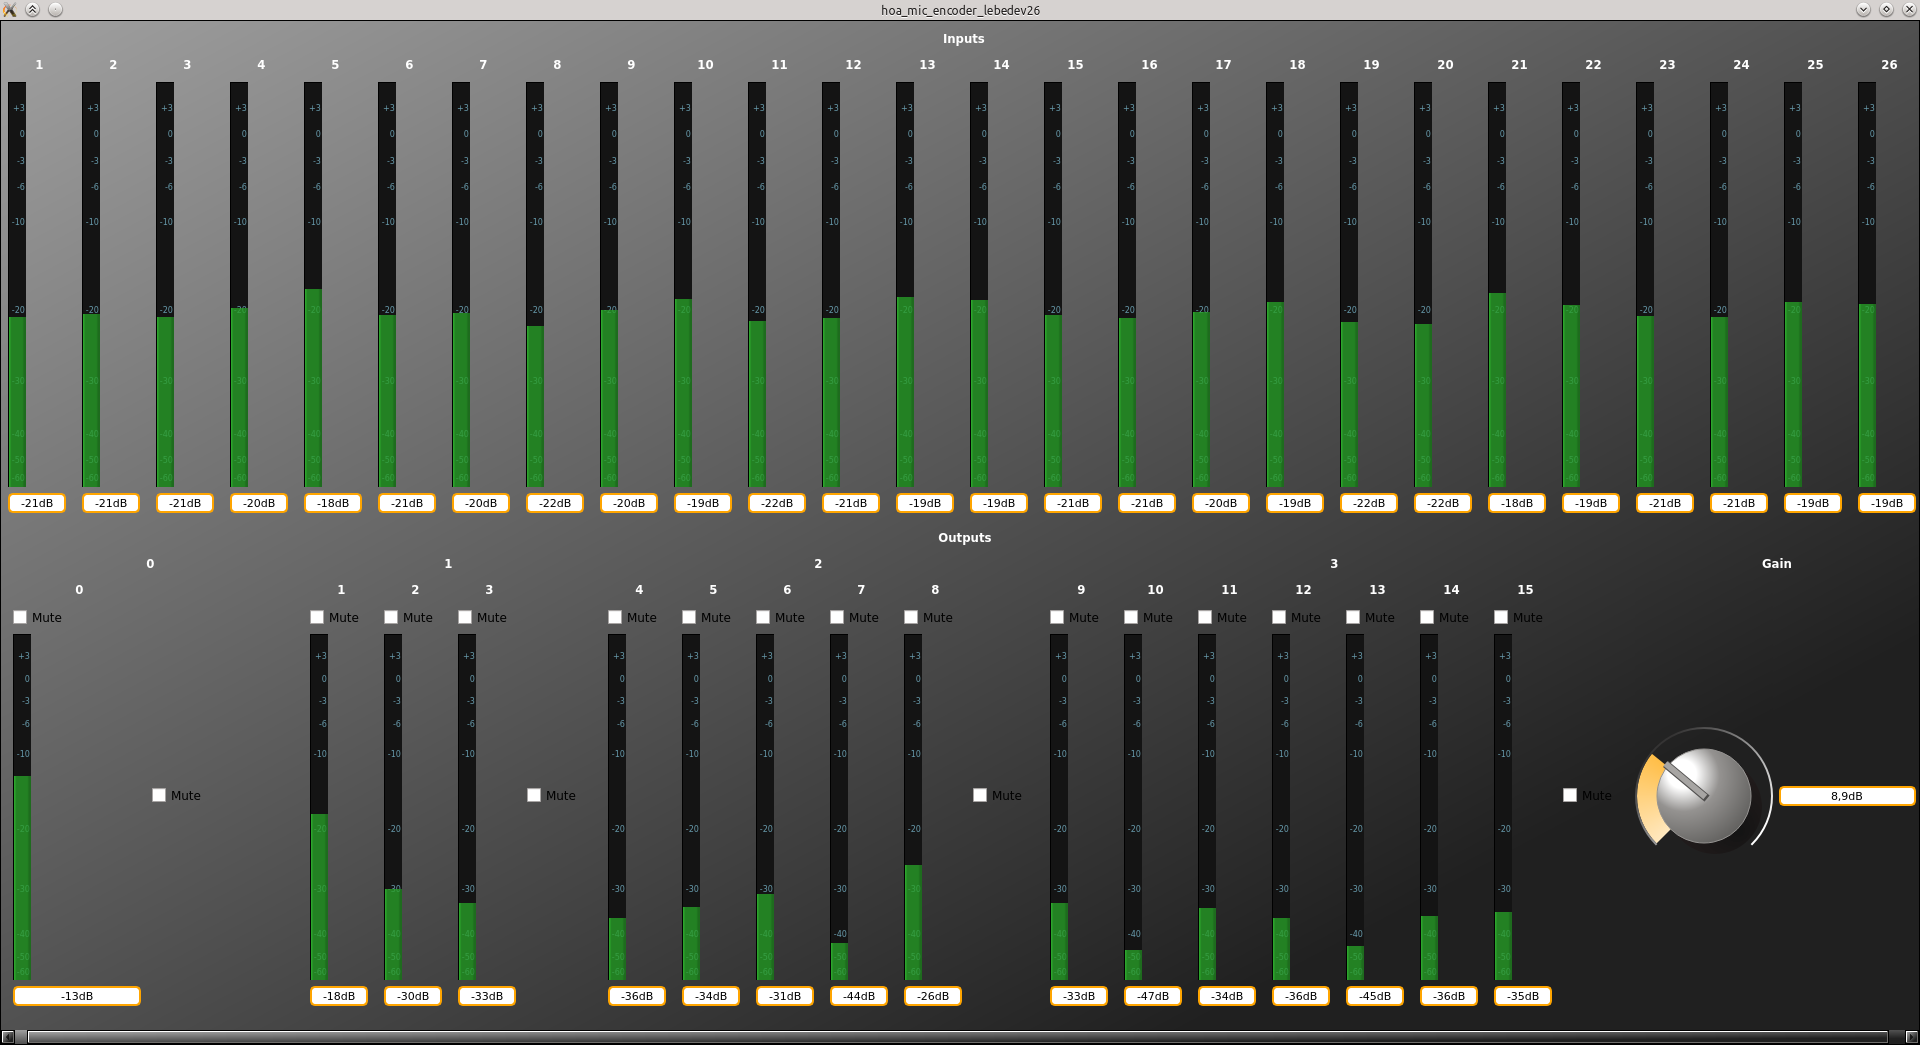
\includegraphics[width=\columnwidth]{hoa_mic_encoder.png}
\caption{\lstinline'hoa_mic_encoder_lebedev26' compiled using \lstinline'faust2jaqt' script with $M=3$. The VU-Meters at the top show the signal level in dBFS of each capsule on the spherical microphone. The VU-Meters at the bottom show the signal level of each components after the DSFT operation. The check-boxes \lstinline'Mute' allow to mute some components or all components of an order. The knob \lstinline'Gain' applies a global gain on the output signals.}
\label{fig:hoa_mic_encoder_lebedev26}
\end{figure}

Fig.~\ref{fig:hoa_mic_encoder_2} shows the connection in order to obtain the Ambisonics components from the signals of a rigid spherical microphone. The raw signals issued from the spherical microphone are played using a Digital Audio Workstation, Ardour 4 in this case. Those signals feed the tool \lstinline'hoa_mic_encoder_lebedev50' in the middle of Fig.~\ref{fig:hoa_mic_encoder_2}. This tool mix the signals to operate the DSFT. The resulting outputs signals are finally filtered using Jconvolver, on the right of Fig.~\ref{fig:hoa_mic_encoder_2}. The outputs of Jconvolver are the Ambisonics components, here up to order $M=5$.
\begin{figure}[!ht]
\centering
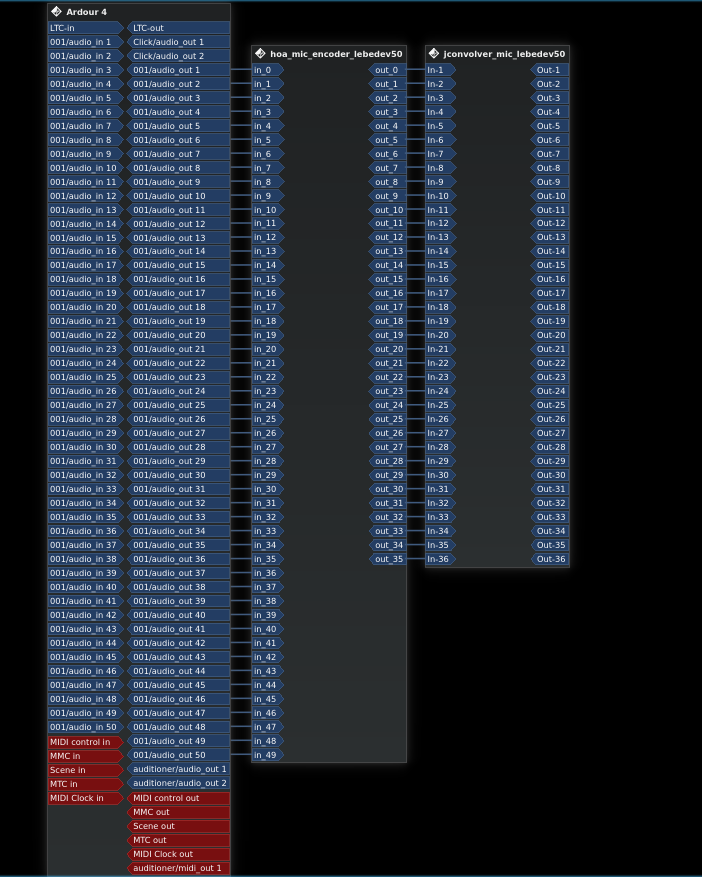
\includegraphics[width=0.75\columnwidth]{hoa_mic_encoder_2.png}
\caption{Connections in order to obtain the Ambisonics components from the signals of a rigid spherical microphone. On the left, the $50$ outputs of Ardour 4: the $50$ signals of the rigid spherical microphone with a $50$-node Lebedev configuration. On the middle, the tool \lstinline'hoa_mic_encoder_lebedev50' which operates the DSFT. On the right, the filtering of the signals with Jconvolver, the outputs of this box are the Ambisonics components up to order $M=5$. Sceen-shot taken from Claudia under KXStudio Linux distribution.}
\label{fig:hoa_mic_encoder_2}
\end{figure}

\pagebreak
\subsubsection{hoa\_decoder\_*}
\label{sec:hoa_decoder}
\begin{itemize}
\item Inputs: $(M+1)^2$
\item Outputs: $06$, $26$ or $50$ depending on the decoder.
\end{itemize}

Three basic decoders by mode-matching \cite{daniel2000representation,poletti2005three} are available at the moment in ambitools: \lstinline'hoa_decoder_lebedev06', \lstinline'hoa_decoder_lebedev26' and
\lstinline'hoa_decoder_lebedev50'. Those decoders allow to decode $(M+1)^2$ Ambisonics signals on Lebedev grids with respectively $6$, $26$ and $50$ loudspeakers \cite{lebedev1975values,lecomte2015on}. Those grids are able to reconstruct the sound field up to order $M=1$, $M=3$ and $M=5$ respectively.
If other decoders are required, you should have a look at the ambisonic decoder toolbox from Aaron Heller \cite{heller2012toolkit}, or contact me. The graphical user interface when using \lstinline'faust2jaqt' script is shown in Fig.~\ref{fig:hoa_decoder_lebedev50} for the \lstinline'hoa_decoder_lebedev50' decoder compiled with $M=5$. The decoder can be with or without near-field compensation (NFC) filters \cite{daniel2003further,lecomte2015real}. Those filters allow to take into account the finite distance of the loudspeakers: In other terms, if they are disabled, the loudspeakers are modeled as plane-wave generators. In case of spherical wave encoding using the \lstinline'hoa_N_sources_encoder' plug-in, the \lstinline'NFC' check-box should be unchecked as the near-field compensation filters are already used at encoding step (see Sec.~\ref{sec:hoa_encoder}).
\begin{figure}[!ht]
\includegraphics[width=\columnwidth]{hoa_decoder_lebedev50.png}
\caption{\lstinline'hoa_decoder_lebedev50' compiled using \lstinline'faust2jaqt' script with $M=5$. The slider \lstinline'Outputs Gain' applies a global gain on all outputs (loudspeakers signals). The slider \lstinline'Inputs Gain' applies a global gain on all inputs ($B$-Format signals). The VU-Meters \lstinline'Inputs' and \lstinline'Outputs' give the signals level in dBFS. The check-box \lstinline'NFC' activate or deactivate the near-field compensation filters. The input entry \lstinline'Speakers Radius' allows to set the spherical grid radius. Finally, the check-boxes \lstinline'Mute' above all inputs VU-meters allow to mute some specific $B$-Format signals. Or, all the signal from an order with \lstinline'Mute' check-boxes on side of a VU-Meter group.}
\label{fig:hoa_decoder_lebedev50}
\end{figure}

\paragraph{Usage with the Spherical VU-Meter}
Note that when using these tools to drive the Spherical VU-Meter (Sec.~\ref{sec:processing}) with OSC, you need to activate OSC transmission mode 2. This is done by launching the tool with the argument \lstinline'-xmit 2'. For example, with the decoder \lstinline'hoa_decoder_lebedev50', the command should be:
\begin{lstlisting}
$ ./hoa_decoder_lebedev50 -xmit 2
\end{lstlisting}
\pagebreak

\subsubsection{hoa\_decoder\_lebedev50\_binaural}
\begin{itemize}
\item Inputs: $(M+1)^2$
\item Outputs: 2
\end{itemize}
\pagebreak

\subsubsection{hoa\_panning\_*}
\label{section:hoa_panning}
\begin{itemize}
\item Inputs: $N$
\item Outputs: $06$, $26$ or $50$ depending on the configuration.
\end{itemize}

It is possible to compute directly the signals of the loudspeakers without passing by an encoding and decoding process \cite{lecomte2015on}. This equivalent 3D-panning is implemented in the tools \\ \lstinline'hoa_panning_N_sources_lebedev06', \lstinline'hoa_panning_N_sources_lebedev26' and \\ \lstinline'hoa_panning_N_sources_lebedev50' for Lebedev grids with $6$, $26$ and $50$ loudspeakers respectively \cite{lebedev1975values,lecomte2015on}. Those grids allow to control the sound field up to order $M=1$, $M=3$ and $M=5$ respectively \cite{lecomte2015on}. 
The graphical user interface when using \lstinline'faust2jaqt' script is shown in Fig.~\ref{fig:hoa_panning_N_sources_lebedev50} for the \lstinline'hoa_panning_N_sources_lebedev50' panning tool compiled with $M=5$ and $N=2$.
\begin{figure}[!ht]
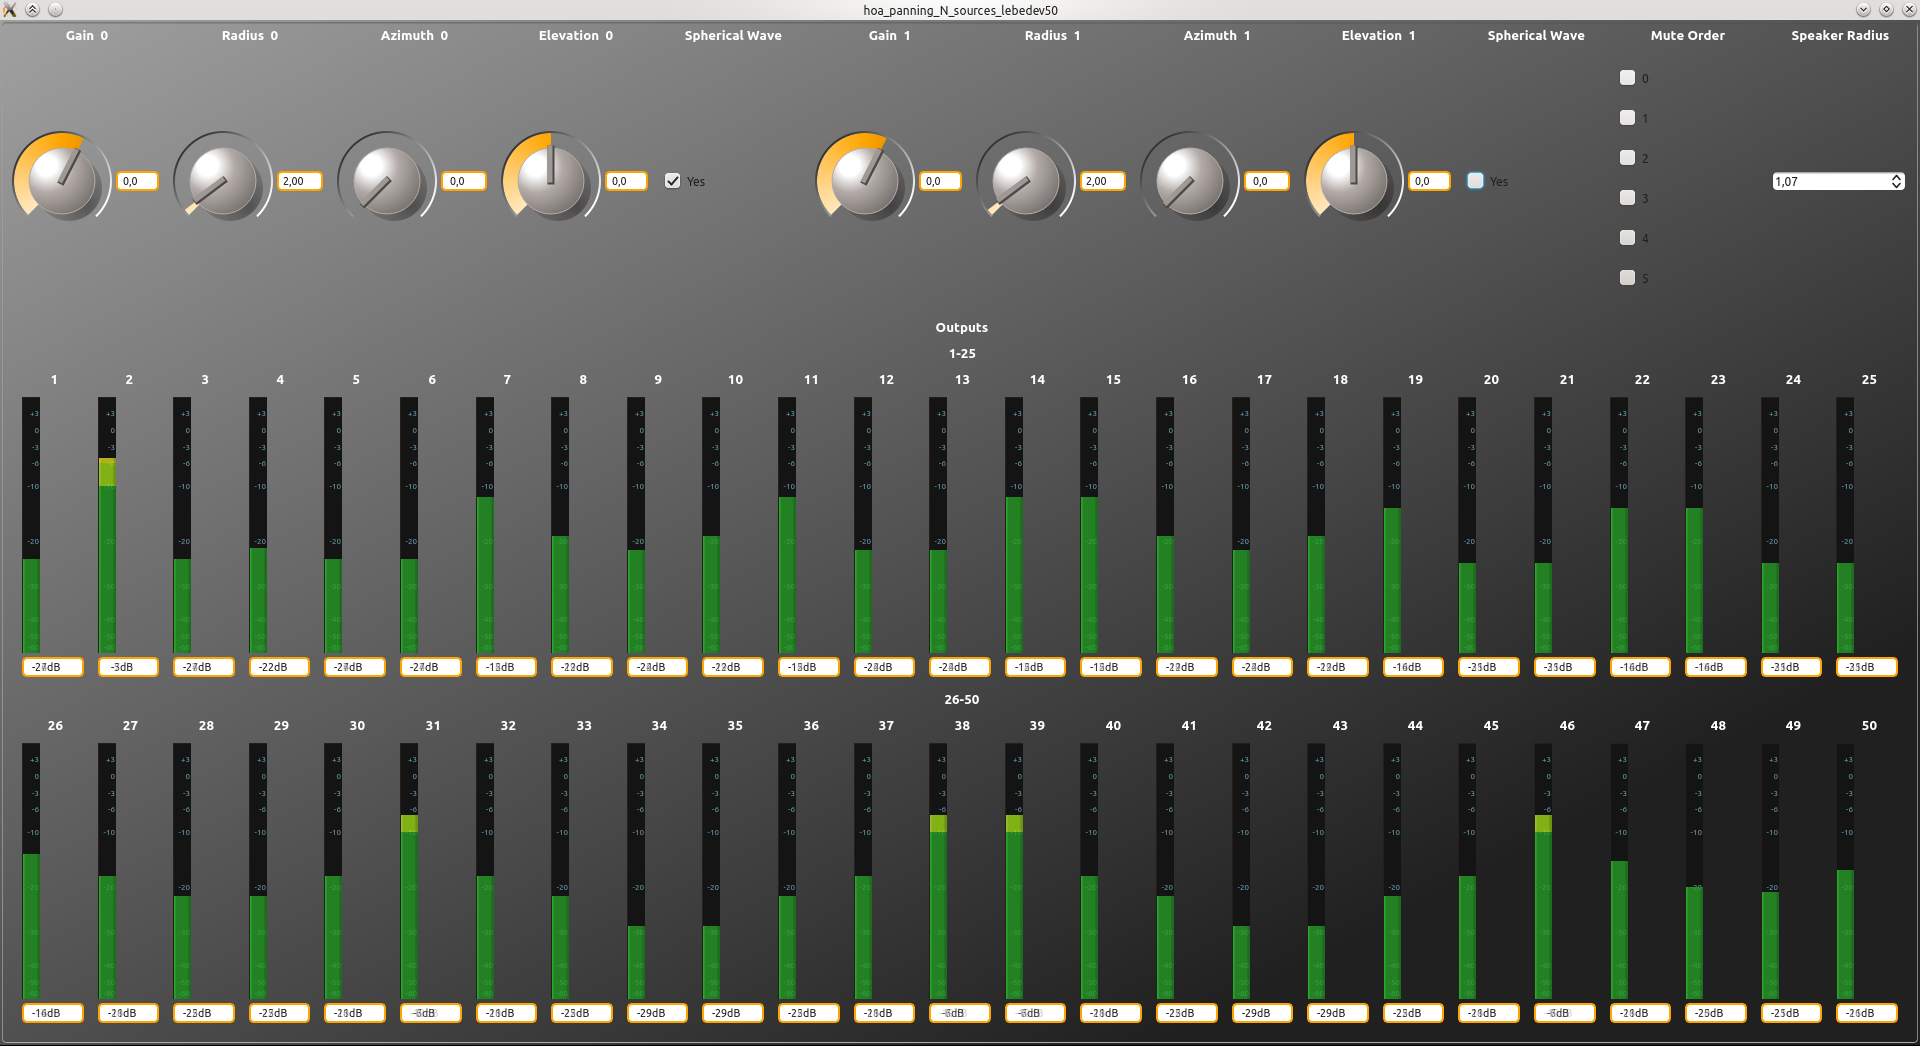
\includegraphics[width=\columnwidth]{hoa_panning_lebedev50.png}
\caption{\lstinline'hoa_panning_N_sources_lebedev50' compiled using \lstinline'faust2jaqt' script with $M=5$ and $N=2$. The slider \lstinline'Outputs Gain' applies a global gain on all outputs (loudspeakers signals). The check-boxes \lstinline'Mute Order' allow to mute some Ambisonic order in the computation of the driving signals. The sliders \lstinline'Gain' \lstinline'Radius' \lstinline'Azimuth' \lstinline'Elevation' control the position and gain of the sources. The check-box \lstinline'Spherical Wave' allows to switch between the synthesis of a spherical wave or a plane wave. In the case of spherical wave synthesis, the input entry \lstinline'Speakers Radius' sets the spherical loudspeakers system radius.}
\label{fig:hoa_panning_N_sources_lebedev50}
\end{figure}
\paragraph{Usage with the Spherical VU-Meter}
Note that when using these tools to drive the Spherical VU-Meter (Sec.~\ref{sec:processing}) with OSC, you need to activate OSC transmission mode 2. This is done by launching the tool with the argument \lstinline'-xmit 2'. For example, with the panning tool \lstinline'hoa_panning_N_sources_lebedev50', the command should be:
\begin{lstlisting}
$ ./hoa_panning_N_sources_lebedev50 -xmit 2
\end{lstlisting}
\pagebreak

\subsubsection{Note about sound field transformation tools in Ambisonic domain}
The tools presented in the next sections perform sound field transformations in Ambisonic domain. Thus, they should be used on Ambisonic signals and inserted after encoding step and before decoding step. For instance, on Fig.~\ref{fig:hoa_mirroring_claudia} is shown the connections for the tool \lstinline'hoa_mirroring': It is inserted after \lstinline'hoa_encoder_N_sources' and before \lstinline'hoa_decoder_lebedev50', acting on Ambisonic signals.
\begin{figure}[!ht]
\centering
\includegraphics[width=0.75\columnwidth]{hoa_mirroring_claudia.png}
\caption{Connections between plug-ins \lstinline'hoa_encoder_N_sources',  \lstinline'hoa_mirroring' and \lstinline'hoa_decoder_lebedev50' compiled with \lstinline'faust2jaqt' script with $M=5$. \lstinline'hoa_mirroring' acts on Ambisonics signals. Screen-shot taken from Claudia under KXStudio Linux distribution.}
\label{fig:hoa_mirroring_claudia}
\end{figure}

\pagebreak
\subsubsection{hoa\_mirroring}
\begin{itemize}
\item Inputs: $(M+1)^2$
\item Outputs: $(M+1)^2$
\end{itemize}
\lstinline'hoa_mirroring' performs mirroring operations on the sound field. The directions front and back can be inverted, as well as left and right, up and down, or any combination of the above. In fact, the transformation changes the sign of particular Ambisonic components \cite{kronlachner2014spatial}. The graphical user interface when using \lstinline'faust2jaqt' script is shown in Fig.~\ref{fig:hoa_mirroring}. To "visualize" the transformation, Fig.~\ref{fig:hoa_mirroring_2} shows the Spherical VU-Meter (see Sec.~\ref{sec:processing}) for a 50-node Lebedev grid with a source positioned at $(1.07~\text{m}, 0^\circ, 90^\circ)$, i.e, above the head of the listener. One can observe the signal level of each loudspeaker after decoding step. Thus, on Fig.~\ref{fig:hoa_mirroring_2a}, when the \lstinline'hoa_mirroring' tool is not active, the maximum sound energy is above. When the check-box \lstinline'up-down' is checked, on Fig.~\ref{fig:hoa_mirroring_2b} one observes that the sound field has been mirrored according to the up-down inversion. Thus, the sound energy is coming from under the listener at present.
\begin{figure}[!ht]
\centering
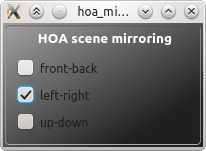
\includegraphics[width=0.3\columnwidth]{hoa_mirroring.png}
\caption{\lstinline'hoa_mirroring' compiled using \lstinline'faust2jaqt' script. The check-boxes allows to select the mirror transformations among: \lstinline'left-right', \lstinline'front-back' or \lstinline'up-down'.}
\label{fig:hoa_mirroring}
\end{figure}
\begin{figure}[!ht]
\centering
\subfigure[]{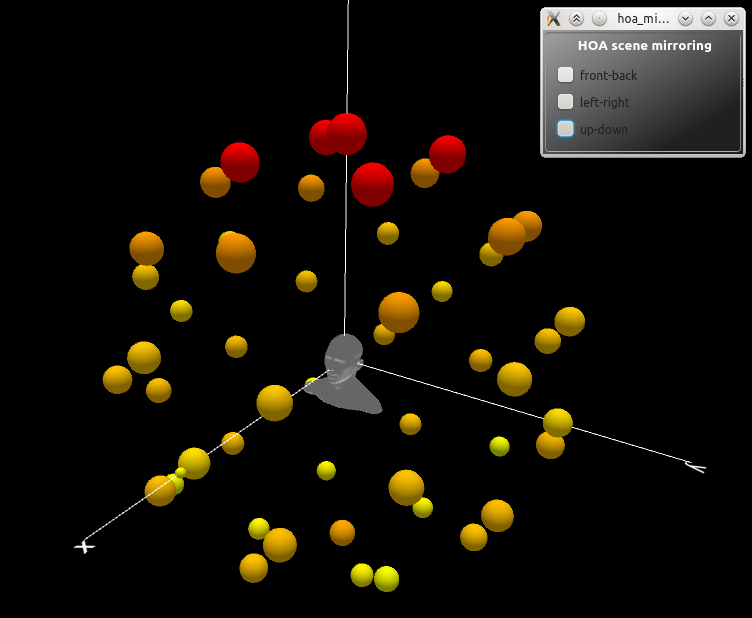
\includegraphics[width=0.45\columnwidth]{hoa_mirroring_2.png}
\label{fig:hoa_mirroring_2a}}
\subfigure[]{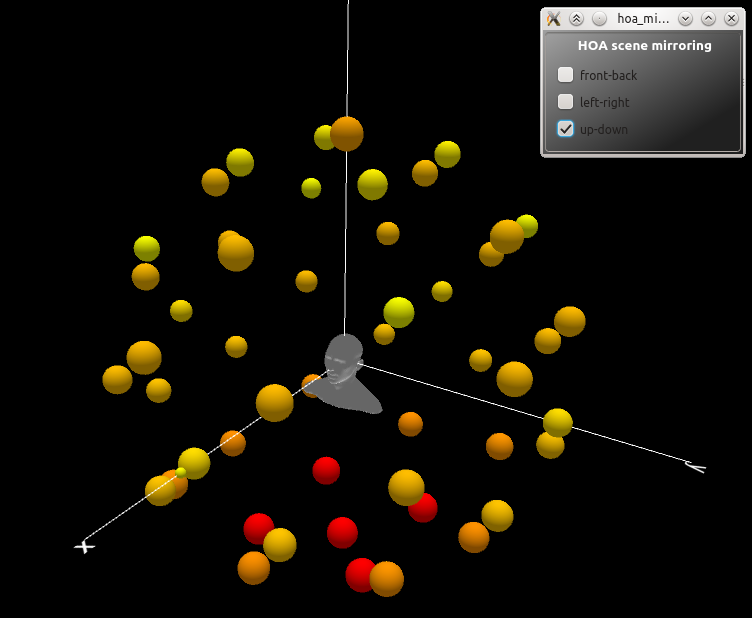
\includegraphics[width=0.45\columnwidth]{hoa_mirroring_3.png}
\label{fig:hoa_mirroring_2b}}
\caption{\lstinline'hoa_mirroring' effects on a sound field. \subref{fig:hoa_mirroring_2a}: original sound field decoded on a 50 loudspeaker Lebedev grid. \subref{fig:hoa_mirroring_2b} the sound field has been transformed according to a mirroring up-down with \lstinline'hoa_mirroring' tool.}
\label{fig:hoa_mirroring_2}
\end{figure}


\pagebreak
\subsubsection{hoa\_azimuth\_rotator}
\begin{itemize}
\item Inputs: $(M+1)^2$
\item Outputs: $(M+1)^2$
\end{itemize}
\lstinline'hoa_azimuth_rotator' performs a rotation of the sound field around $z-$axis (yaw angle). One recalls that the trigonometric sens is chosen for rotation convention (i.e. anti-clockwise) (see Sec.~\ref{sec:spherical_coordinates}). The transformation is done by a rotation matrix operation on the Ambisonic components \cite{daniel2000representation, moreau2006etude,kronlachner2014spatial}. The graphical user interface when using \lstinline'faust2jaqt' script is shown in Fig.~\ref{fig:hoa_azimuth_rotator}. It's basically just a slider to choose the azimuth angle of rotation. To "visualize" the transformation, Fig.~\ref{fig:hoa_azimuth_rotator_2} shows the Spherical VU-Meter (see Sec.~\ref{sec:processing}) for a 50-node Lebedev grid with a source positioned at $(1.07~\text{m}, 0^\circ, 0^\circ)$, i.e, in front of the listener. One can observe the signal level of each loudspeaker after decoding step. Thus, on Fig.~\ref{fig:hoa_mirroring_2a}, when the \lstinline'hoa_azimuth_rotator' slider \lstinline'Azimuth' is set to $0^\circ$, i.e. no rotation, the maximum sound energy is in front of the listener. When the slider \lstinline'Azimuth' is set to $90^\circ$, on Fig.~\ref{fig:hoa_mirroring_2b} one observes that the sound field has been rotated $90^\circ$ counter-clockwise around the $z-$axis. Thus, the sound energy is coming from the left of the listener at present.
\begin{figure}[!ht]
\centering
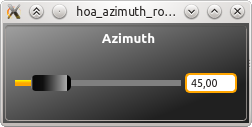
\includegraphics[width=0.3\columnwidth]{hoa_azimuth_rotator.png}
\caption{\lstinline'hoa_azimuth_rotator' compiled using \lstinline'faust2jaqt' script. The slider \lstinline'Azimuth' allows to choose the azimuth angle of rotation, around the $z-$axis.}
\label{fig:hoa_azimuth_rotator}
\end{figure}
\begin{figure}[!ht]
\centering
\subfigure[]{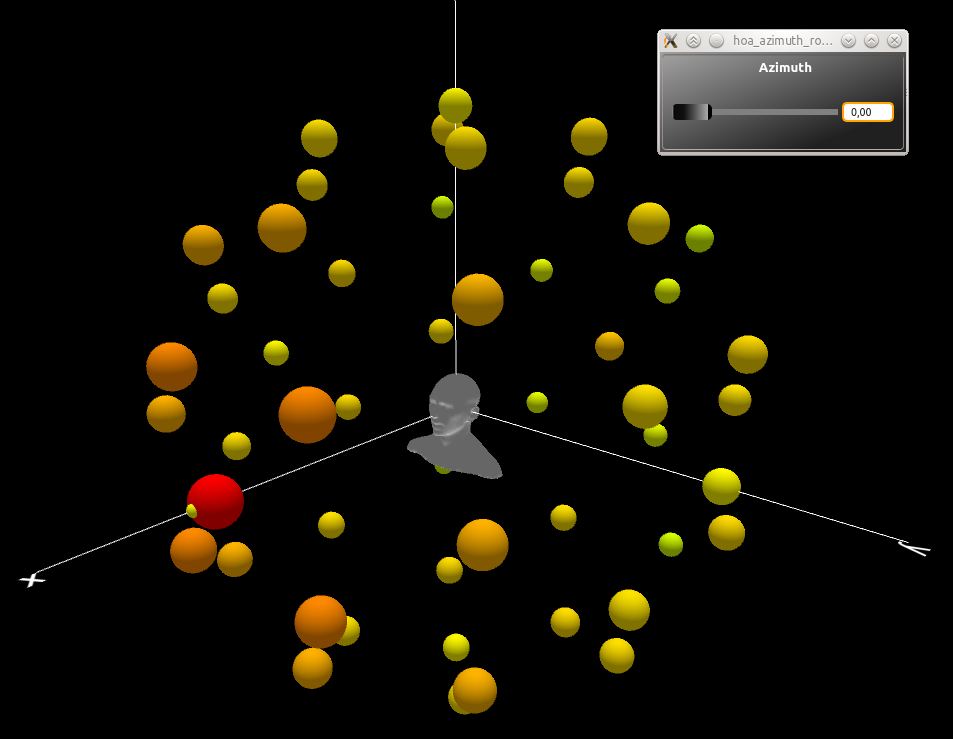
\includegraphics[width=0.45\columnwidth]{hoa_azimuth_rotator2.png}
\label{fig:hoa_azimuth_rotator_2a}}
\subfigure[]{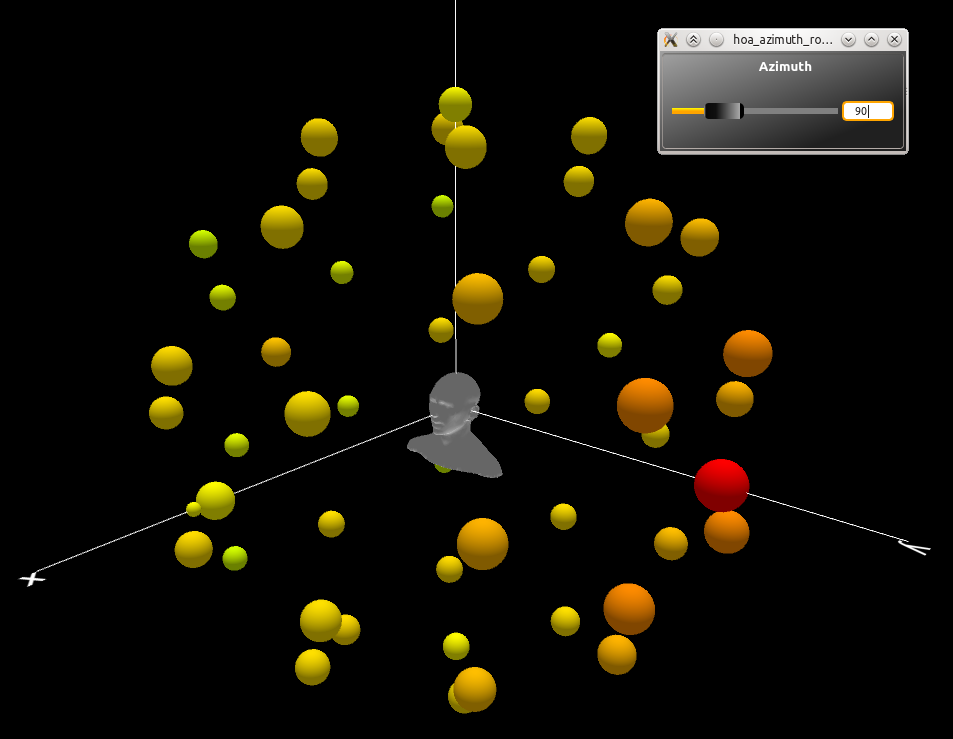
\includegraphics[width=0.45\columnwidth]{hoa_azimuth_rotator3.png}
\label{fig:hoa_azimuth_rotator_2b}}
\caption{\lstinline'hoa_azimuth_rotator' effects on a sound field. \subref{fig:hoa_azimuth_rotator_2a}: original sound field decoded on a 50 loudspeaker Lebedev grid. \subref{fig:hoa_azimuth_rotator_2b} the sound field has been rotated according to a rotation around $z-$axis of $+90^\circ$ using \lstinline'hoa_azimuth_rotator' tool.}
\label{fig:hoa_azimuth_rotator_2}
\end{figure}
\paragraph{Head Tracking}
One possible use of the tool \lstinline'hoa_azimuth_rotator' is to compensate the rotation of the head of the listener around $z-$axis when driven by a head-tracking system \cite{noisternig20033d}. Thus, when using binaural rendering over headphone, the sound field is rotated of minus the angle of rotation of the head, to compensate the head rotation and leave the source at the same position is space for the listener. ambitools provides a Pure Data patch to drive \lstinline'hoa_azimuth_rotator' with OSC and perform an cheap head-tracking system with a smart-phone. See Sec.~\ref{sec:andOSC} for further informations.

\pagebreak
\subsubsection{hoa\_beamforming\_hypercardioid\_to\_mono}
\begin{itemize}
\item Inputs: $(M+1)^2$
\item Output: $1$
\end{itemize}
\lstinline'hoa_beamforming_hypercardioid_to_mono' is a tool to perform modal beamforming and extract a monophonic signal as if it was recorded by a directional microphone in the sound field. In fact, the Ambisonic signals are weighted and summed to give the monophonic output signal. The weights of the combination traduce the beampattern of the directional microphone which is used \cite{meyer2002highly}. Thus, this tool allows to listen to a chosen direction in the 3D sound field as if you were recording in the middle of the sound field with a directional microphone with a specific beampattern. \lstinline'hoa_beamforming_hypercardioid_to_mono' provides the weights corresponding to regular hyper-cardioid microphone up to order $3$ \cite{meyer2002highly,lecomte2016filtrage}. On Fig.~\ref{fig:hoa_beamforming_hypercardioids}, the beampatterns available are shown: the higher the order of the hyper-cardioid is, the more directional the corresponding virtual microphone becomes. The graphical user interface when using \lstinline'faust2jaqt' script is shown in Fig.~\ref{fig:hoa_beamforming_hypercardioid_to_mono} for $M=3$.
\begin{figure}[!ht]
\centering
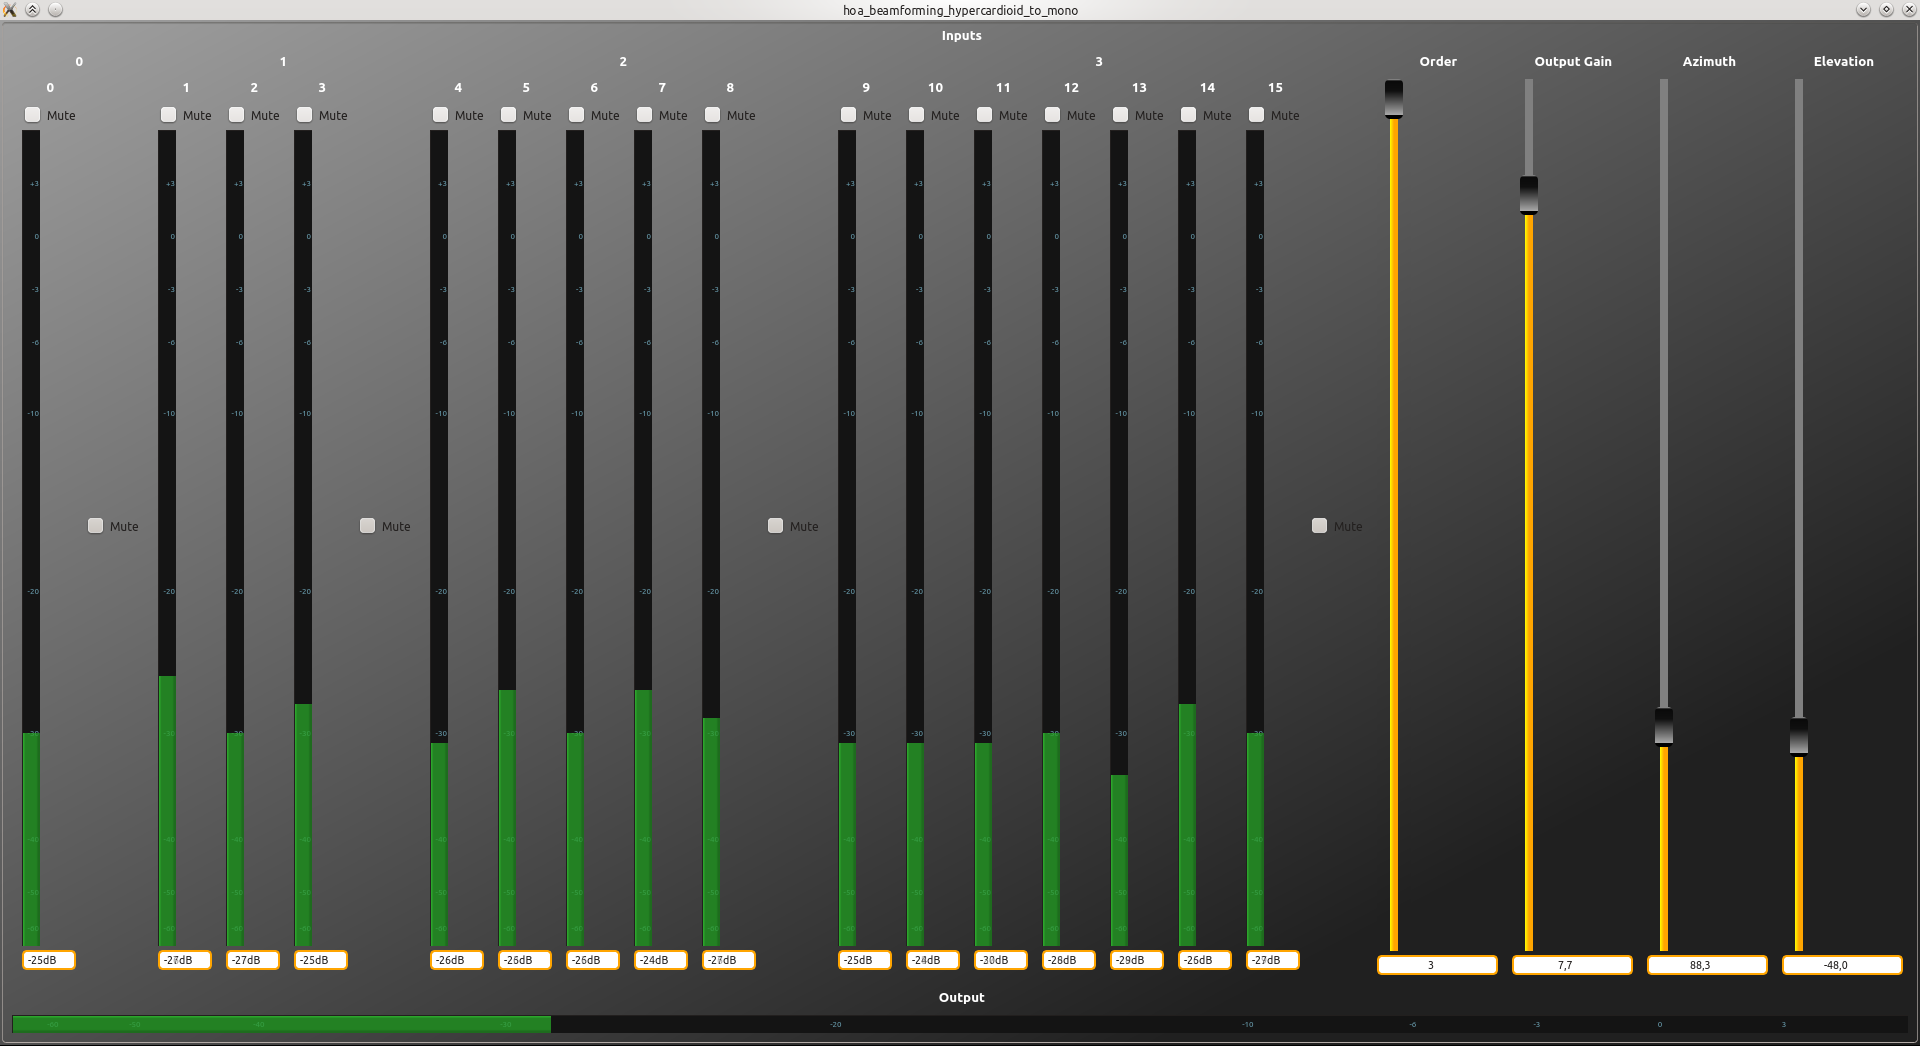
\includegraphics[width=\columnwidth]{hoa_beamforming_hypercardioid_to_mono.png}
\caption{\lstinline'hoa_beamforming_hypercardioid_to_mono' compiled using \lstinline'faust2jaqt' script. The VU-Meters on the left give the signal level of each Ambisonic component. The check-boxes \lstinline'Mute' allow to mute some components of all the components of an order. On the right, the slider \lstinline'Order' allows to select the regular hyper-cardioid order. The slider \lstinline'Output Gain' applies a gain on the output signal. The sliders \lstinline'Azimuth' and \lstinline'Elevation' allow to set the steering angles $(\theta_0,\delta_0)$ of the hyper-cardioid beampattern. Finally, the horizontal VU-Meter on bottom shows the output signal level.}
\label{fig:hoa_beamforming_hypercardioid_to_mono}
\end{figure}
\begin{figure}[!ht]
\subfigure[Order 1]{
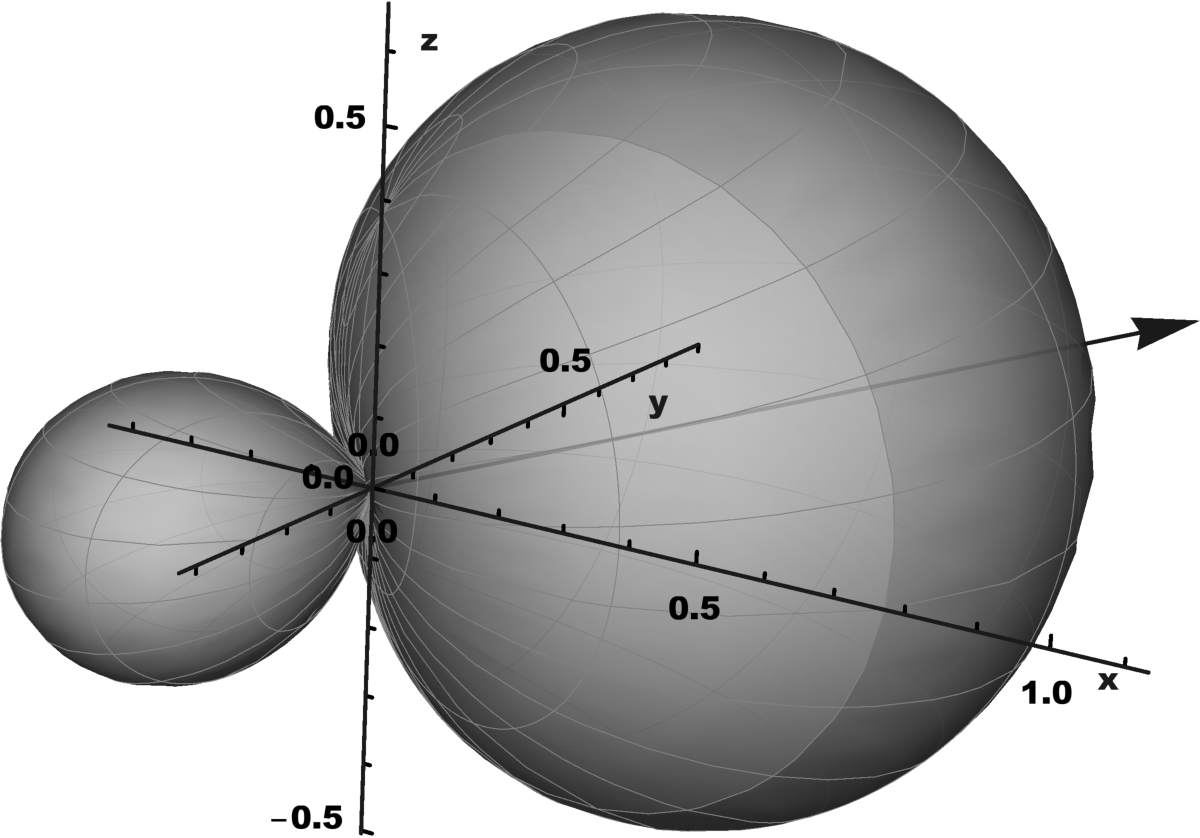
\includegraphics[width=0.3\columnwidth]{hypercardioid1.pdf}
\label{fig:hoa_beamforming_hypercardioid_1}
}
\subfigure[Order 2]{
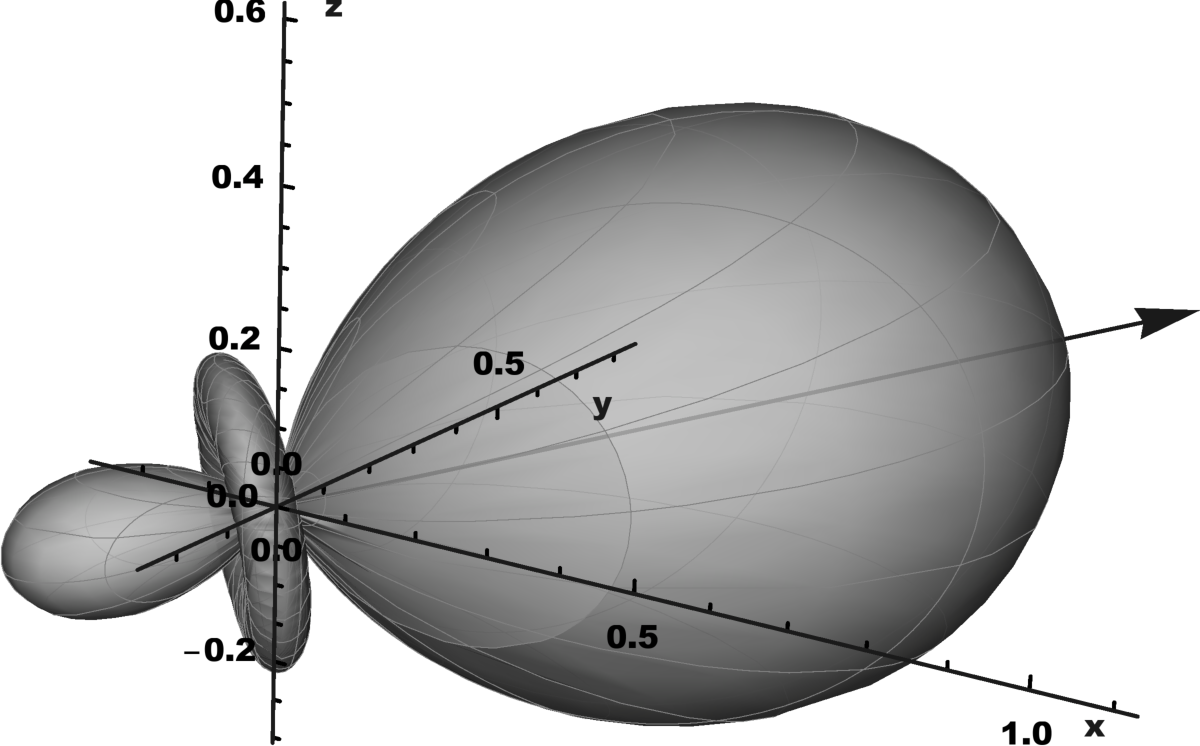
\includegraphics[width=0.3\columnwidth]{hypercardioid2.pdf}
\label{fig:hoa_beamforming_hypercardioid_2}
}
\subfigure[Order 3]{
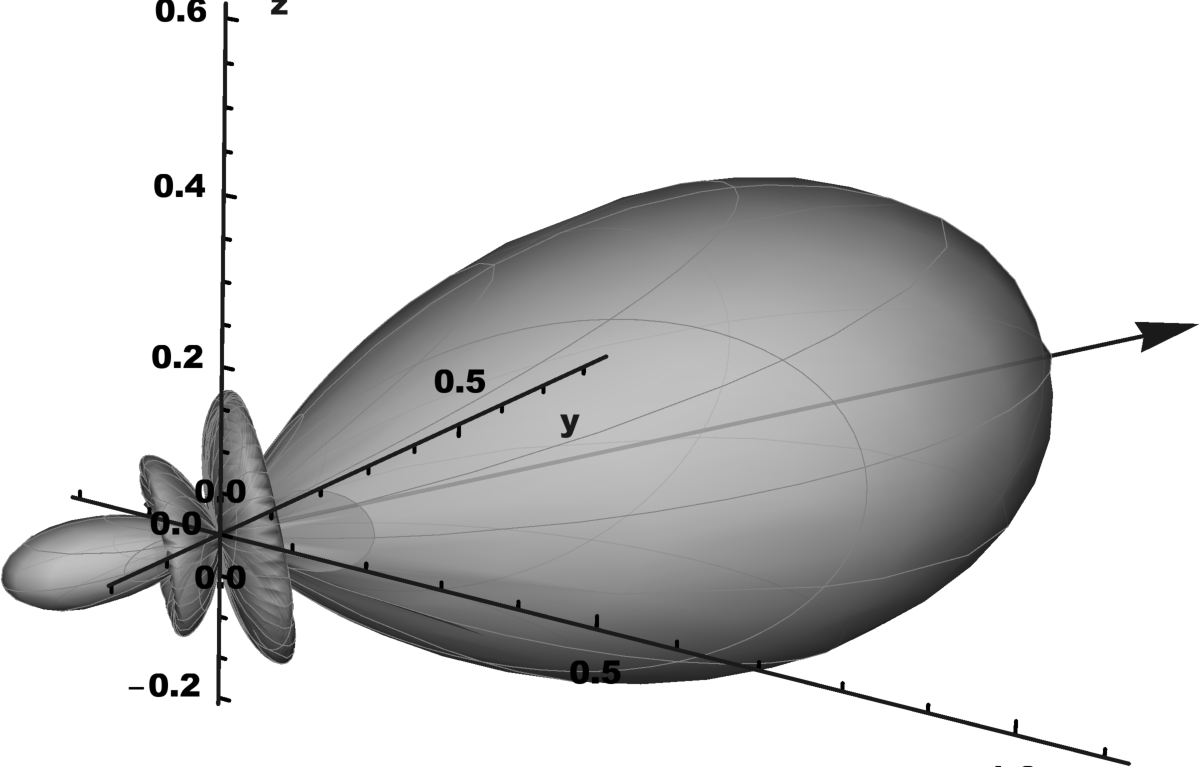
\includegraphics[width=0.3\columnwidth]{hypercardioid3.pdf}
\label{fig:hoa_beamforming_hypercardioid_3}
}
\caption{Regular hyper-cardioid beampattern up to order 3. The steering angles are $(\theta_0 = 45^\circ, \delta_0=10^\circ)$.}
\label{fig:hoa_beamforming_hypercardioids}
\end{figure}

\subsubsection{hoa\_beamforming\_hypercardioid\_to\_hoa}
\subsubsection{hoa\_beamforming\_dirac\_to\_hoa}

\pagebreak
\subsection{Processing}
\subsubsection{Spherical\_VU\_Meter}
\label{sec:processing}
ambitools provides a Spherical VU-Meter developped with \textsc{Processing} language. A screen-shot is shown on Fig.~\ref{fig:spherical_vu_meter}. This tool allows to "see" where the sound energy is in space, instead of using classical in-line VU-Meter. You can zoom, pan and rotate the view of the meter while running. The \textsc{Faust} tools \lstinline'hoa_panning*' and \lstinline'hoa_decoder*' emit \textsc{OSC} messages on port UDP 5511. Those messages drive the spherical VU-Meter rendering in real-time: loudspeakers size and color for the meter, and source position.
\begin{figure}[!ht]
\centering
\includegraphics[width=\columnwidth]{spherical_vu_meter.png}
\caption{\lstinline'Spherical_VU_Meter' for a 50 loudspeaker Lebedev array and two virtual sources. Each loudspeaker is represented as a color ball with size and color proportional to RMS Level in dBFS. A scale in dBFS is displayed on the left of the screen. The virtual sources are represented as red an yellow dots. Their coordinates are displayed in Cartesian and spherical coordinates on the left. A grey manikin is standing in the middle of the array to indicates the front direction.}
\label{fig:spherical_vu_meter}
\end{figure}

\pagebreak
\subsection{Jconvolver}
\label{sec:jconvolver}
\subsubsection{jconvolver\_mic*}
\subsubsection{hrir\_lebedev50}

\subsection{Pure Data}
\subsubsection{andOSC.pd for Head Tracking}
\label{sec:andOSC}
\subsubsection{joyscick\_XYZ\_to\_OSC.pd to control Faust tools with a Joystick}
\subsubsection{houseflushell.pd to generate the sound of flies}

\section{Examples of use}
\subsubsection{Listening to a 3D HOA recording through binaural rendering}
\subsubsection{Spatialize and control the trajectories of flies}
%\subsection{Record trajectories with Ardour}
\bibliography{These,ATIAM,Livres}
\bibliographystyle{apalike}

\end{document}
